\documentclass[11pt]{article}
\usepackage{amsmath}
\usepackage{graphicx}

\setlength{\parindent}{0pt}
\setlength{\parskip}{0.7em}
\setlength{\textwidth}{6.5in}
\setlength{\oddsidemargin}{0in}
\setlength{\evensidemargin}{0in}
\setlength{\topmargin}{-0.4in}
\setlength{\textheight}{9.2in}

\begin{document}

\begin{center}
{\Large SYSC 5108 Exam Study: Assignment 1, Question 5}\\
\vspace{0.3em}
{\large Linear regression, Newton update, quadratic regression, and capacity}\\
\vspace{0.3em}
Source question: \texttt{SYSC 5108 W26 Assignment 1.pdf}, Question 5
\end{center}

\section*{Question Setup}

The dataset is
\[
\begin{array}{c|ccccc}
\text{sample} & 1 & 2 & 3 & 4 & 5\\
\hline
x & 0.1 & 1.3 & 3.5 & 6.4 & 8.9\\
y & -1.2 & 2.7 & 1.4 & 4.3 & 2.6
\end{array}
\]
The third sample point, $(3.5, 1.4)$, is the test point. The remaining four points are the training data:
\[
(0.1,-1.2),\quad (1.3,2.7),\quad (6.4,4.3),\quad (8.9,2.6).
\]

The main reference is Chapter 2 slides 4--5: write the linear model in matrix form, minimize summed squared error, and solve with
\[
\beta^*=(X^T X)^{-1}X^T y.
\]
For part (e), use Chapter 2 slide 10:
\[
\nabla_\beta L(\beta)=-2X^T(y-X\beta), \qquad
\beta_{\text{new}}=\beta-\epsilon \nabla_\beta L(\beta).
\]
This also matches Goodfellow, Bengio, and Courville, \textit{Deep Learning}, Chapter 5, Section 5.1.4 on linear regression and mean squared error.

\section*{Part (a): Optimal Linear Regression Model}

Use the model
\[
\hat y=\beta_0+\beta_1x.
\]
For the four training points,
\[
X=
\begin{bmatrix}
1 & 0.1\\
1 & 1.3\\
1 & 6.4\\
1 & 8.9
\end{bmatrix},
\qquad
y=
\begin{bmatrix}
-1.2\\
2.7\\
4.3\\
2.6
\end{bmatrix}.
\]
Compute
\[
X^T X=
\begin{bmatrix}
4 & 16.7\\
16.7 & 121.87
\end{bmatrix},
\qquad
X^T y=
\begin{bmatrix}
8.4\\
54.05
\end{bmatrix}.
\]
Then
\[
\beta^*=(X^T X)^{-1}X^T y
=
\begin{bmatrix}
0.5804353\\
0.3639676
\end{bmatrix}.
\]
Therefore the fitted line is
\[
\boxed{\hat y=0.5804+0.3640x.}
\]

Now test on $(x,y)=(3.5,1.4)$:
\[
\hat y(3.5)=0.5804353+0.3639676(3.5)=1.8543219.
\]
The squared test error is
\[
SE=(y-\hat y)^2=(1.4-1.8543219)^2=0.2064084.
\]
So
\[
\boxed{SE_{\text{linear}} \approx 0.2064.}
\]

\begin{figure}[h]
\centering
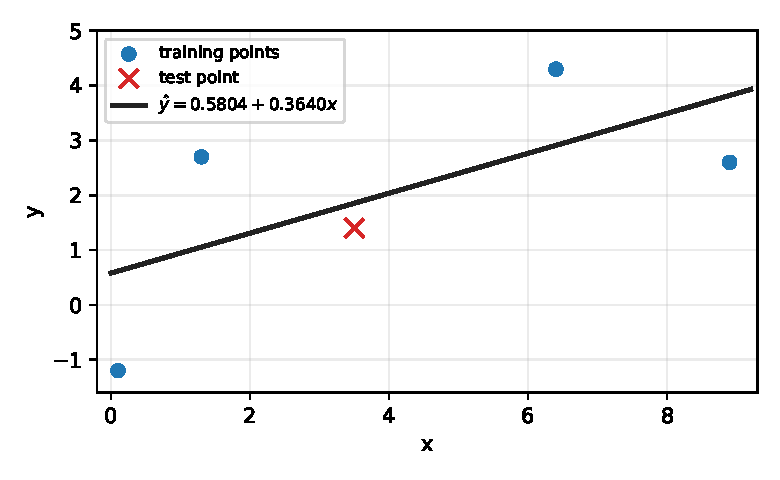
\includegraphics[width=0.78\textwidth]{a1_q5_linear_fit.pdf}
\caption{Linear fit using samples 1, 2, 4, and 5 as training data; sample 3 is the test point.}
\end{figure}

\section*{Part (b): Newton's Method from $\beta=(0,0)^T$}

For summed squared error,
\[
L(\beta)=(y-X\beta)^T(y-X\beta),
\]
the gradient and Hessian are
\[
g(\beta)=\nabla_\beta L(\beta)=2X^T(X\beta-y),
\qquad
H=2X^T X.
\]
At
\[
\beta_0=
\begin{bmatrix}
0\\
0
\end{bmatrix},
\]
we get
\[
g(\beta_0)=
\begin{bmatrix}
-16.8\\
-108.1
\end{bmatrix},
\qquad
H=
\begin{bmatrix}
8 & 33.4\\
33.4 & 243.74
\end{bmatrix}.
\]
Newton's method uses the curvature-corrected direction:
\[
\beta_{\text{new}}=\beta_0-\epsilon H^{-1}g(\beta_0).
\]
Because this loss is a quadratic function of $\beta$, the exact Newton step reaches the minimizer in one step. Therefore the optimal Newton step length is
\[
\boxed{\epsilon^*=1.}
\]
Thus
\[
\beta_{\text{new}}
=
\begin{bmatrix}
0\\
0
\end{bmatrix}
-
1\cdot
H^{-1}
\begin{bmatrix}
-16.8\\
-108.1
\end{bmatrix}
=
\begin{bmatrix}
0.5804353\\
0.3639676
\end{bmatrix}.
\]
So Newton's method gives the same answer as part (a):
\[
\boxed{\hat\beta_{\text{Newton}}=
\begin{bmatrix}
0.5804\\
0.3640
\end{bmatrix}.}
\]

\textbf{Important exam note.} If instead one uses the steepest-descent line-search formula from Chapter 2 slide 8 along the raw negative-gradient direction, then
\[
\epsilon_{\text{SD}}^*
=
\frac{g^Tg}{g^THg}
=0.004027,
\]
and one gradient descent step from zero gives only
\[
\beta_1=
\begin{bmatrix}
0.0677\\
0.4353
\end{bmatrix}.
\]
That is not the same as the Newton answer because steepest descent and Newton's method use different directions. Since the assignment asks for Newton's method, the relevant step length is $\epsilon^*=1$.

\section*{Part (c): Optimal Quadratic Regression Model}

Use the quadratic model
\[
\hat y=\beta_0+\beta_1x+\beta_2x^2.
\]
The expanded design matrix is
\[
X_q=
\begin{bmatrix}
1 & 0.1 & 0.01\\
1 & 1.3 & 1.69\\
1 & 6.4 & 40.96\\
1 & 8.9 & 79.21
\end{bmatrix},
\qquad
y=
\begin{bmatrix}
-1.2\\
2.7\\
4.3\\
2.6
\end{bmatrix}.
\]
Using the same normal equation,
\[
\beta_q^*=(X_q^T X_q)^{-1}X_q^T y
=
\begin{bmatrix}
-0.7687718\\
2.2253109\\
-0.2107787
\end{bmatrix}.
\]
Therefore
\[
\boxed{\hat y=-0.7688+2.2253x-0.2108x^2.}
\]

Now test on $(x,y)=(3.5,1.4)$:
\[
\hat y(3.5)
=-0.7687718+2.2253109(3.5)-0.2107787(3.5)^2
=4.4377768.
\]
The squared test error is
\[
SE=(1.4-4.4377768)^2=9.2280881.
\]
So
\[
\boxed{SE_{\text{quadratic}} \approx 9.2281.}
\]

\begin{figure}[h]
\centering
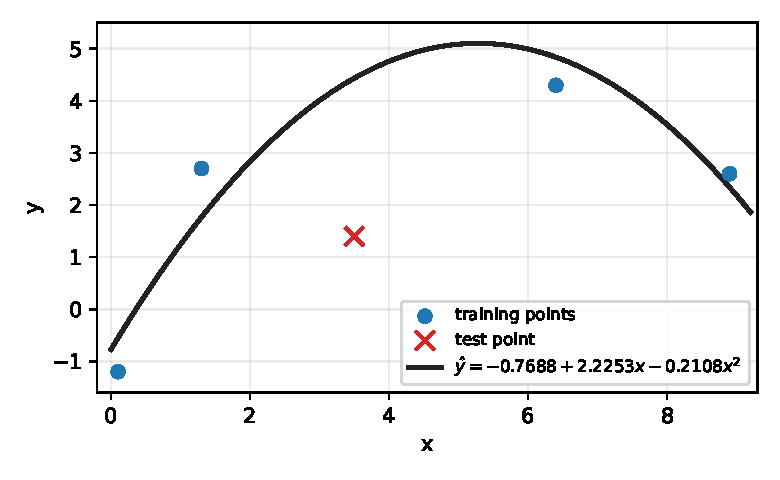
\includegraphics[width=0.78\textwidth]{a1_q5_quadratic_fit.pdf}
\caption{Quadratic fit using samples 1, 2, 4, and 5 as training data; sample 3 is the test point.}
\end{figure}

\section*{Part (d): Compare Errors and Discuss Capacity}

The linear model's test squared error is
\[
SE_{\text{linear}}\approx 0.2064,
\]
while the quadratic model's test squared error is
\[
SE_{\text{quadratic}}\approx 9.2281.
\]
The quadratic model has much worse test error on the held-out point.

This is a capacity example. Chapter 2 slide 24 defines capacity as the ability to fit a wide variety of functions, and gives polynomials as an example of expanding the hypothesis space beyond ordinary linear regression. The quadratic model has higher capacity because it can bend. Here, that extra flexibility reduces the training summed squared error:
\[
SSE_{\text{train, linear}}\approx 9.4319,\qquad
SSE_{\text{train, quadratic}}\approx 1.6520.
\]
However, it generalizes worse to the test point:
\[
SE_{\text{test, linear}}\approx 0.2064,\qquad
SE_{\text{test, quadratic}}\approx 9.2281.
\]
This illustrates the training/generalization tradeoff from Chapter 2 slides 23--25 and Goodfellow et al., Chapter 5, Section 5.2: lower training error does not guarantee lower test error. Increasing capacity can help when the simpler model underfits, but it can also overfit when there is too little data.

\section*{Part (e): One Gradient/Backward-Propagation Update}

Use the linear model with
\[
\beta=
\begin{bmatrix}
0.80\\
0.60
\end{bmatrix},
\qquad
\epsilon=0.001.
\]
The model predictions on the four training points are
\[
X\beta=
\begin{bmatrix}
0.86\\
1.58\\
4.64\\
6.14
\end{bmatrix}.
\]
The residual vector is
\[
y-X\beta=
\begin{bmatrix}
-2.06\\
1.12\\
-0.34\\
-3.54
\end{bmatrix}.
\]
The summed squared error at the initialized parameter is
\[
L(\beta)=(-2.06)^2+(1.12)^2+(-0.34)^2+(-3.54)^2=18.1452.
\]
The gradient is
\[
\nabla_\beta L(\beta)=-2X^T(y-X\beta)
=
\begin{bmatrix}
9.6400\\
64.8640
\end{bmatrix}.
\]
Apply one update:
\[
\beta_{\text{new}}
=
\beta-\epsilon\nabla_\beta L(\beta)
=
\begin{bmatrix}
0.80\\
0.60
\end{bmatrix}
-0.001
\begin{bmatrix}
9.6400\\
64.8640
\end{bmatrix}
=
\begin{bmatrix}
0.79036\\
0.535136
\end{bmatrix}.
\]
So the one-step update is
\[
\boxed{
\beta_{\text{new}}
=
\begin{bmatrix}
0.7904\\
0.5351
\end{bmatrix}.}
\]

\section*{Cross References Used}

\begin{itemize}
\item Assignment: \texttt{SYSC 5108 W26 Assignment 1.pdf}, Question 5.
\item Local submitted Assignment 1 PDF checked for comparison, Question 5 response.
\item Slides: Chapter 2 slide deck, slides 4--5 on linear regression, least squares, and prediction error.
\item Slides: Chapter 2 slide deck, slide 8 on gradient descent step size and curvature.
\item Slides: Chapter 2 slide deck, slide 10 on gradient descent for linear regression and backward error propagation.
\item Slides: Chapter 2 slide deck, slides 23--25 on training error, generalization error, capacity, and overfitting.
\item Textbook: Goodfellow, Bengio, and Courville, \textit{Deep Learning}, Chapter 4, Sections 4.3 and 4.5 on gradient-based optimization and linear least squares.
\item Textbook: Goodfellow, Bengio, and Courville, \textit{Deep Learning}, Chapter 5, Sections 5.1.4 and 5.2 on linear regression, mean squared error, generalization, underfitting, and overfitting.
\end{itemize}

\end{document}
